\documentclass[9pt,aspectratio=43,mathserif,table]{beamer} 
%  设置为 Beamer 文档类型,设置字体为 10pt,长宽比为16:9,数学字体为 serif 风格
\batchmode
\usepackage{graphicx}
\usepackage{subfigure}
\usepackage{fontspec}
\usepackage{amsmath}

% \setmainfont{Harding Text Web Regular Regular.ttf}
\usepackage{diagbox} % 表头斜线分区
\usepackage{unicode-math}
\usefonttheme{serif}
% \setmathrm{Harding Text Web Regular Regular.ttf} % 设置数学字体为 Times New Roman
\setmathfont{TeX Gyre Termes Math} % 如果您使用 XeLaTeX 或 LuaLaTeX 编译,可以使用其他数学字体
\setmathtt{Courier New} % 设置等宽字体为 Courier New
\setboldmathrm{Times New Roman}
\setmathfont{TeX Gyre Termes Math}[version=bold] % 设置粗体数学字体
\setmathfont{TeX Gyre Termes Math}[range={\mathit}]


\usetheme{Berlin} %主题
\setbeamertemplate{page number in head/foot}[pagenumber]
%\usecolortheme{sustech} %主题颜色

\usepackage[ruled,linesnumbered]{algorithm2e}

\usepackage{fancybox}
\usepackage{xcolor}
\usepackage{listings}

\usepackage{booktabs}
\usepackage{colortbl}

\newcommand{\Console}{Console}
\lstset{ %
	backgroundcolor=\color{white},   % choose the background color
	basicstyle=\footnotesize\rmfamily,     % size of fonts used for the code
	columns=fullflexible,
	breaklines=true,                 % automatic line breaking only at whitespace
	captionpos=b,                    % sets the caption-position to bottom
	tabsize=4,
	commentstyle=\color{mygreen},    % comment style
	escapeinside={\%*}{*)},          % if you want to add LaTeX within your code
	keywordstyle=\color{blue},       % keyword style
	stringstyle=\color{mymauve}\ttfamily,     % string literal style
	numbers=left, 
	%	frame=single,
	rulesepcolor=\color{red!20!green!20!blue!20},
	% identifierstyle=\color{red},
	language=c
}


\definecolor{mygreen}{rgb}{0,0.6,0}
\definecolor{mymauve}{rgb}{0.58,0,0.82}
\definecolor{mygray}{gray}{.9}
\definecolor{mypink}{rgb}{.99,.91,.95}
\definecolor{mycyan}{cmyk}{.3,0,0,0}

%题目,作者,学校,日期
\title{Conservative Systems \& Reversible Systems}
%\subtitle{\fontsize{9pt}{14pt}\textbf{跨临界分岔}}
\author{Speaker: Yichen Lu\quad \newline  \newline \quad }
\institute{\fontsize{8pt}{14pt}}
\date{\today}
\newcommand{\concept}{Conservative Systems \& Reversible Systems}

%学校Logo
%\pgfdeclareimage[height=0.5cm]{sustech-logo}{sustech-logo.pdf}
%\logo{\pgfuseimage{sustech-logo}\hspace*{0.3cm}}

\AtBeginSection[]
{
	\begin{frame}<beamer>
	\frametitle{\textbf{Contents}}
	\tableofcontents[currentsection]
\end{frame}
}
% \beamerdefaultoverlayspecification{<+->}
% -----------------------------------------------------------------------------
\begin{document}
% -----------------------------------------------------------------------------

\frame{\titlepage}

% \section[Contents]{}   %目录
% \begin{frame}{Contents}
% \tableofcontents
% \end{frame}

% -----------------------------------------------------------------------------
\section{Conservative Systems}

\begin{frame}{Conservative Systems}
    \begin{align*}
		m\ddot{x}&=F(x)\\
		m\ddot{x}+\frac{dV}{dx}&=0 \quad \left(F(x)=-\frac{dV}{dx}\right)\\
		m\dot{x}\ddot{x}+\frac{dV}{dx}\dot{x}&=0 \quad \left(\text{multiply both sides by } \dot{x}\right)\\
		\frac{d}{dt}\left[\frac{1}{2}m\dot{x}^2+V(x)\right]&=0 \quad \left(\frac{d}{dt}V(x(t))=\frac{dV}{dx}\frac{dx}{dt}\right)\\
		\frac{dE}{dt}&=0 \quad \left(E=\frac{1}{2}m\dot{x}^2+V(x)\right)
	\end{align*}
	% 很多重要二阶系统都是源自牛顿定律F=ma, 这里我们就拿一个例子来介绍保守系统,假设一个质子在力F的作用下运动,m是质量,x是位置,V是势能。我们假设F关于dot x和t是独立的,并且没有任何摩擦力等阻力,切驱动力F不随时间变化,我们在这些假设下,我们可以发现这个系统的能量守恒的。在这里,我们定义F是势能V的负变化量,这样我们就可以得到一个关于x的势能函数V,这个函数是x的二阶函数,为了化简它这里有一个窍门是两边同时乘dot x,再逆用链式法则,我们就可以得到一个关于t的函数,这个函数就是能量E,我们可以看到E关于t的导数是0,也就是说E不随时间t变化,那么这个系统就是保守系统。

	Systems for which a conserved quantity exists are called \textbf{conservative systems}.

\end{frame}

\begin{frame}
	% 下面来更严格地定义保守系统
	\begin{itemize}
		\item A conserved quantity is a real-valued continuous function $E(x)$ that is constant on trajectories, i.e. $dE/dt = 0$
		% 如果存在一个实值连续函数E(x),这个函数在轨迹上是常数,也就是说E关于t的导数是0,那么这个量就是一个守恒量,一个具有守恒量的系统就是保守系统。
		\item To avoid trivial examples, we also require that $E(x)$ be nonconstant on every open set.
		% 为了避免平凡的例子,我们还要求E(x)在每个开集上都是非常数的。否则,如果E(x)是常数,那么E(x)就是一个平凡的守恒量,这样的守恒量是没有意义的。
		\item A conservative system cannot have any attracting fixed points.
		% 保守系统不能有任何吸引的不动点,因为如果有吸引的不动点,那么根据吸引子的定义,存在一个足够小的邻域,这个邻域内的轨迹都会收敛到这个不动点,又因为E(x)是常数,所以这个邻域内的轨迹都是常数,那么这个不动点附近的这个邻域,也就是这个开集上,E(x)是常数,这样就和我们的定义矛盾了。保守系统的这一性质在后面的例题中非常重要
		\begin{figure}
			\centering
			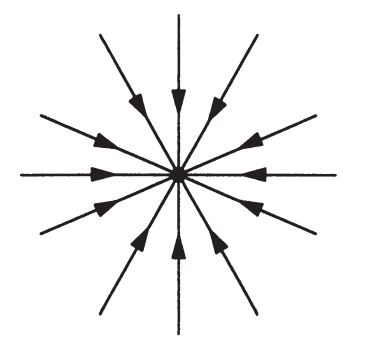
\includegraphics[width=0.35\linewidth]{attractingFixedPoints.png}
		\end{figure}
	\end{itemize}
\end{frame}

\begin{frame}
	% 除了吸引不动点不存在,保守系统中还有其他的不动点,在接下来的例题中,我们对鞍点和中心点的存在性进行分析
	$$
	V(x)=-\frac{1}{2}x^2+\frac{1}{4}x^4
	$$
	Since $F=-\frac{dV}{dx}=x-x^3$, $\ddot{x}=x-x^3$
	$$
	% 由于力是势能的负变化量,所以力是x-x^3,那么加速度就是x-x^3,这个系统的运动方程可以写成这个
	\begin{cases}
		\dot{x}=y\\
		\dot{y}=x-x^3\\
	\end{cases}
	$$
	% 可以容易求得这个系统的不动点,根据雅克布矩阵可以求得不动点的类型,判断得到原点是鞍点,1和-1是中心点
	Fix points: Saddle point: $(0,0)$, Centers: $(\pm 1,0)$

	\begin{figure}
		\centering
		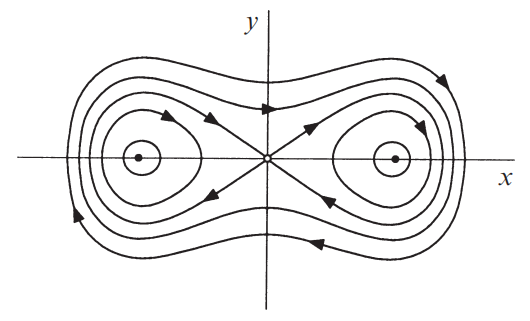
\includegraphics[width=0.4\linewidth]{fig651.png}
	\end{figure}	
	% 这个系统的相图如下图所示,图中的轨迹都是不同的E值的轨迹,在轨迹上移动的点势能都是恒定的,因此可以把他们看作是等高线
	Trajectories that start and end at the same fixed point are called homoclinic orbits.
	% 这里有一种比较特殊的轨道,我们把这种从出发点和终点都为同一不动点的轨道,称为同宿轨
\end{frame}

\begin{frame}

	\begin{columns}
		\begin{column}{0.3\textwidth}
			\begin{figure}
				\centering
				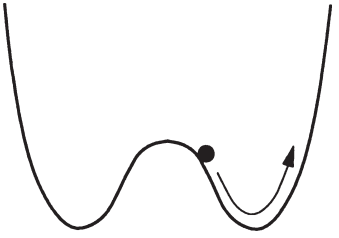
\includegraphics[width=\linewidth]{fig652.png}
			\end{figure}
		\end{column}
		\begin{column}{0.7\textwidth}  %%<--- here
			\begin{figure}
				\centering
				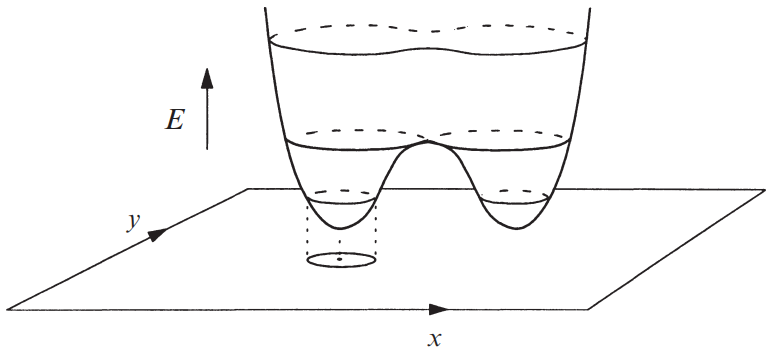
\includegraphics[width=\linewidth]{fig653.png}
			\end{figure}
		\end{column}
	\end{columns}

	The energy $E$ is plotted above each point $( x, y )$ of the phase plane. The resulting surface is often called the energy surface for the system.
	% 这里我们把每个点的能量E画在相平面上,这样得到的曲面,称为能量曲面。这样得到的图像更直观,因为它可以直观地看出轨迹的形状,而且可以看出轨迹的形状和能量的关系,这里我们可以看到,能量越大,轨迹越大,能量越小,轨迹越小,这是因为能量是轨迹上的点的势能,势能越大,轨迹越大,势能越小,轨迹越小。
\end{frame}

\begin{frame}
	\textbf{Theorem 6.5.1:} (Nonlinear centers for conservative systems) Consider the 
	system $\dot{\mathrm{x}}=f(\mathrm{x})$ , where $\mathrm{x}=(x, y)\in R^2$
	, and $f$ is continuously differentiable. Suppose there exists a conserved quantity $E (x)$ and suppose that $x^*$ is an isolated fixed point (i.e., there are no other fixed points in a small neighborhood surrounding $x^*$). If $x^*$ is a local minimum of E, then all trajectories sufficiently close to $x^*$ are closed.
	% 这里我们来证明一个定理,这个定理是关于保守系统中中心点的存在性,这个定理的条件是,系统中存在一个守恒量E,不动点x*是孤立的,也就是说在x*的邻域内没有其他的不动点,如果x*是E的局部最小值,那么x*附近的轨迹都是闭合的。
	% 证明思路是由于E在轨迹上是恒定的,每一条轨迹都包含在E的等高线上。靠近局部最小值或者局部最大值时,等高线是闭的,所以轨迹也是闭的。
	$$\ $$

	\begin{enumerate}
		\item The theorem is valid for local maxima of E also.
		\item We need to assume that $x^*$ is isolated.
		% 这里我们需要假设不动点x*是孤立的,也就是说在x*的邻域内没有其他的不动点,这个假设是必要的,因为如果不动点x*不是孤立的,那么这个性质将不一定满足
	\end{enumerate}
\end{frame}

\section{Reversible Systems}

\begin{frame}{Reversible Systems}
	$$
	\begin{array}{c}
		\dot{x}=y\\
		\dot{y}=\frac{1}{m}F\left( x \right)\\
	\end{array}
	$$
	% 接下来我们介绍可逆系统,可逆系统是指系统在时间反演和空间反演下不变,也就是说,如果x(t)是系统的一个解,那么-x(-t)也是系统的一个解,如果y(t)是系统的一个解,那么-y(-t)也是系统的一个解。
	$$\ $$
	Make the change of variables $t \rightarrow -t$ and $y \rightarrow -y$: if $(x(t), y(t))$ is a solution, then so is $(x(-t), -y(-t))$

	\begin{figure}
		\centering
		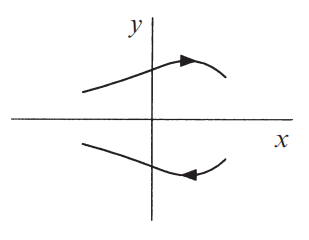
\includegraphics[width=0.4\linewidth]{fig661.jpg}
	\end{figure}

\end{frame}

\begin{frame}
	More generally, let’s define a reversible system to be any second-order system that is invariant under $t \rightarrow -t$ and $y \rightarrow -y$
	$$\ $$
	$$
	\begin{array}{c}
		\dot{x}=f\left( x,y \right)\\
		\dot{y}=g\left( x,y \right)\\
	\end{array}
	$$
	$$\ $$
	where f is odd in y and g is even in y (i.e., $f ( x, -y ) = -f ( x, y )$ and $g ( x, -y ) = g ( x, y )$) is reversible
	% 更一般地,我们定义可逆系统是指系统在时间反演和空间反演下不变,也就是说,如果x(t)是系统的一个解,那么-x(-t)也是系统的一个解,如果y(t)是系统的一个解,那么-y(-t)也是系统的一个解。这里我们定义的可逆系统是指二阶系统,这个系统在时间反演和空间反演下不变。例如,如果f是y的奇函数,g是y的偶函数,也就是说,f(x,-y)=-f(x,y),g(x,-y)=g(x,y),这样的系统是可逆的。
\end{frame}

\begin{frame}
	\textbf{Theorem 6.6.1:} (Nonlinear centers for reversible systems) Suppose the origin $x^* =0$ is a linear center for the continuously differentiable system and suppose that the system is reversible. Then sufficiently close to the origin, all trajectories are closed curves.
	% 和保守系统类似,可逆系统也有中心点的存在性。这个定理内容是,不动点x*是线性中心,系统是可逆的,那么x*附近的轨迹都是闭合的。证明思路是比较简单的,由于x*是中心,所以附近的轨迹都会围绕着x*旋转,另外由于系统是可逆的,所以轨迹是对称的,那么轨迹的一半就是另一半的时间反演,所以轨迹是闭合的。
	$$\ $$

	\begin{columns}
		\begin{column}{0.5\textwidth}
			\begin{figure}
				\centering
				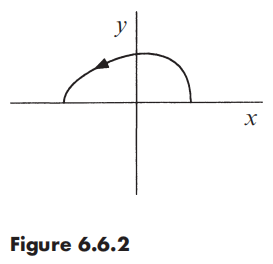
\includegraphics[width=0.6\linewidth]{fig662.jpg}
			\end{figure}
		\end{column}
		\begin{column}{0.5\textwidth}  %%<--- here
			\begin{figure}
				\centering
				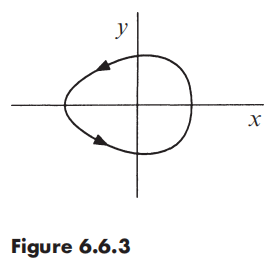
\includegraphics[width=0.6\linewidth]{fig663.jpg}
			\end{figure}
		\end{column}
	\end{columns}	
\end{frame}

\begin{frame}
	$$
	\begin{aligned}
		\dot{x}&=y-y^3\\
		\dot{y}&=-x-y^2\\
	\end{aligned}
	$$
	$$
	A=\left( \begin{matrix}
		\frac{\partial f}{\partial x}&		\frac{\partial f}{\partial y}\\
		\frac{\partial g}{\partial x}&		\frac{\partial g}{\partial y}\\
	\end{matrix} \right) _{\left( 0,0 \right)}=\left( \begin{matrix}
		0&		1\\
		-1&		0\\
	\end{matrix} \right) 
	$$
	\begin{itemize}
		\item $\tau = 0$, $\Delta>0$, so the origin is a linear center.
		\item the system is reversible, since the equations are invariant under the transformation $f ( x, -y ) = -f ( x, y )$ and $g ( x, -y ) = g ( x, y )$
	\end{itemize}
	% 这里我们来看一个例子,在这个系统当中,显然原点是一个不动点,并且根据雅可比矩阵我们可以知道这是一个中心。另外,这个系统是可逆的,因为这个系统在时间反演和空间反演下不变。所以根据定理,原点附近的轨迹都是闭合的。
\end{frame}

\begin{frame}
	% 另外这个系统还有两个不动点,下面是系统的相图,可以看到原点附近的轨迹都是闭合的,另外两个不动点也确实是鞍点
	The other fixed points of the system are $(-1, 1)$ and $(-1, -1)$, they are saddle points.
	\begin{figure}
		\centering
		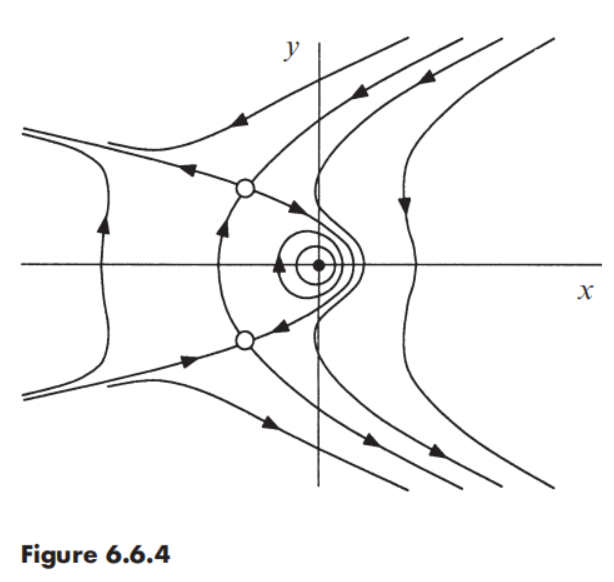
\includegraphics[width=0.5\linewidth]{fig664.jpg}
	\end{figure}
	The twin saddle points are joined by a pair of trajectories, they are called \textbf{heteroclinic trajectories} or \textbf{saddle connections}.
	% 此外,这里成对的鞍点被一对轨迹连接起来。它们被叫作异宿轨道或者鞍形连接
\end{frame}

\begin{frame}
	% 除了可以通过画出相图的方式发现异宿轨道外,异宿轨的存在性可以通过可逆性理论严格地推导出来
	$$
	\begin{aligned}
		\dot{x}&=y\\
		\dot{y}&=x-x^2\\
	\end{aligned}\,\, \left( x>0 \right) \,\,
	$$
	$$
	A=\left( \begin{matrix}
		\frac{\partial f}{\partial x}&		\frac{\partial f}{\partial y}\\
		\frac{\partial g}{\partial x}&		\frac{\partial g}{\partial y}\\
	\end{matrix} \right) _{\left( 0,0 \right)}=\left( \begin{matrix}
		0&		1\\
		1&		0\\
	\end{matrix} \right) 
	$$
	\textbf{Fixed points}: $(0,0)$, saddle point
	One of eigendirection is $v_1=(1,1)$, the other is $v_2=(1,-1)$

	when $0< x < 1$, $\dot{y}=x-x^2>0$, $y$ is increasing, when $x>1$, $\dot{y}=x-x^2<0$, $y$ is decreasing. $\dot{x}=y>0$. Eventually reaching $y = 0$.
	% 这里我们来看一个例子,这个系统的不动点是原点,原点是一个鞍点,这个鞍点的特征向量是1,1和1,-1,这个鞍点的相图如图所示,可以看到,当x>0时,y是增加的,当x<0时,y是减少的,所以轨迹最终会到达y=0的位置。又由系统的可逆性,这里必有一对有相同终点且箭头方向相反的轨迹,此时两条轨迹一起形成同宿轨。
	\begin{columns}
		\begin{column}{0.5\textwidth}
			\begin{figure}
				\centering
				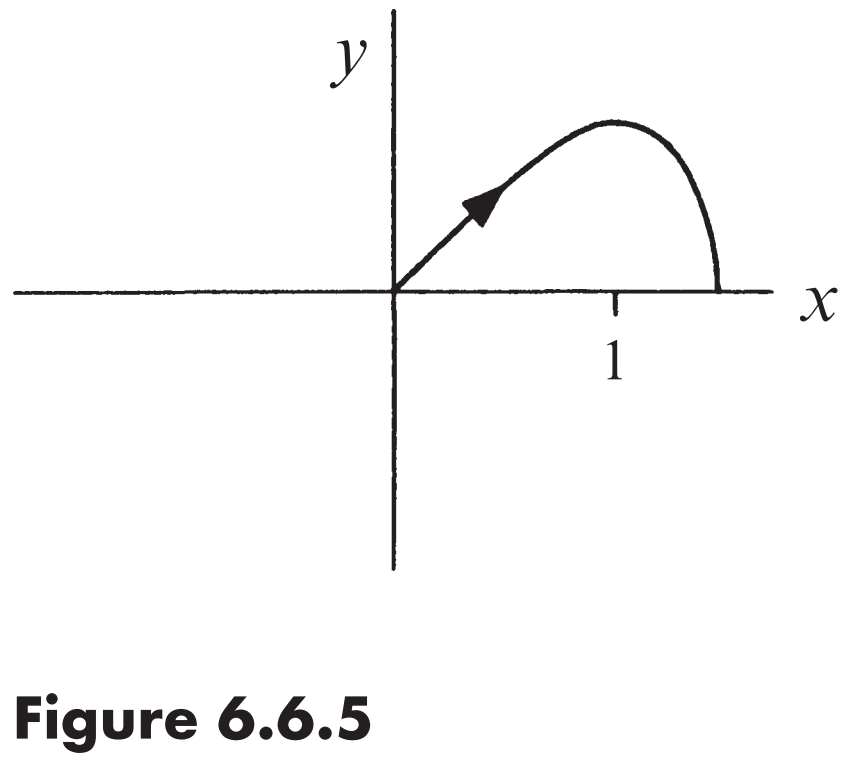
\includegraphics[width=0.6\linewidth]{fig665.jpg}
			\end{figure}
		\end{column}
		\begin{column}{0.5\textwidth}  %%<--- here
			\begin{figure}
				\centering
				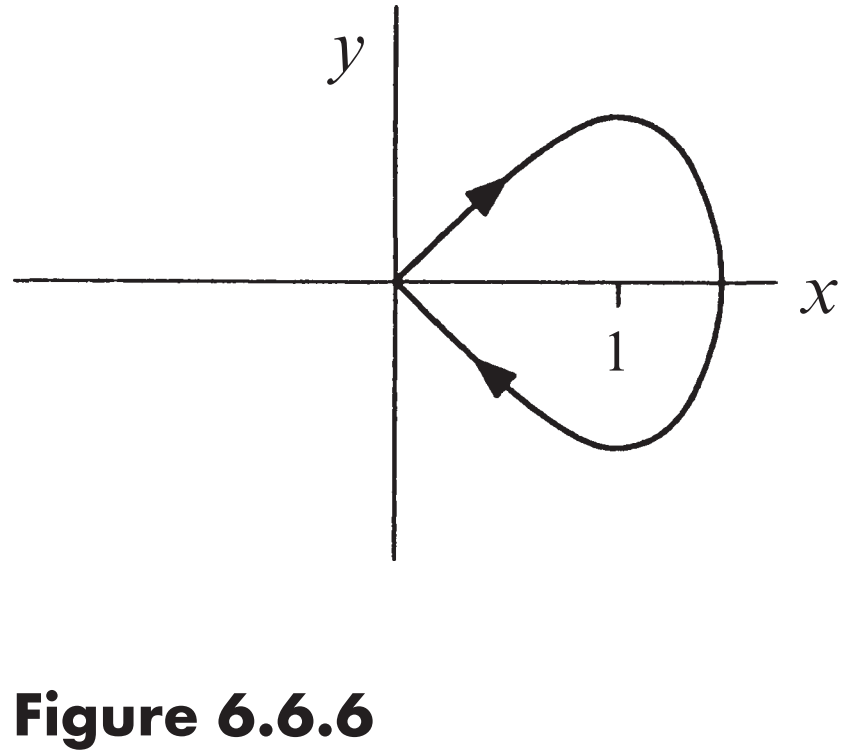
\includegraphics[width=0.6\linewidth]{fig666.jpg}
			\end{figure}
		\end{column}
	\end{columns}
\end{frame}

\begin{frame}
	% 前面介绍了保守系统和可逆系统的相似性,这里以一个例子说明两种系统的不同之处
	$$
	\begin{aligned}
		\dot{x}&=-2\cos x-\cos y\\
		\dot{y}&=-2\cos y-\cos x\\
	\end{aligned}
	$$
	The system is invariant under the change of variables $x \rightarrow -x$, $y \rightarrow -y$ and $t \rightarrow -t$.
	$$
	% 这里我们来看一个例子,这个系统是可逆的,因为这个系统在时间反演和空间反演下不变。接下来我们求这个系统的不动点,可以看到这个系统有四个不动点,其中不动点(-pi/2,-pi/2),根据雅可比矩阵,可以判断它是一个稳定鞍点,也就是吸引子,前面根据定义可知一个保守系统是不含吸引子的,所以这个系统不是保守系统。
	\cos x^*=\cos y^*=0,\left( x^*,y^* \right) =\left( \pm \frac{\pi}{2},\pm \frac{\pi}{2} \right) 
	$$
	$$
	A=\left( \begin{matrix}
		2\sin x&		\sin y\\
		\sin x&		2\sin y\\
	\end{matrix} \right) _{\left( -\frac{\pi}{2},-\frac{\pi}{2} \right)}=\left( \begin{matrix}
		-2&		-1\\
		-1&		-2\\
	\end{matrix} \right) 
	$$
	$\tau=-4, \Delta=3, \tau^2-4\Delta=4$, the fixed point is a stable node.
	\begin{figure}
		\centering
		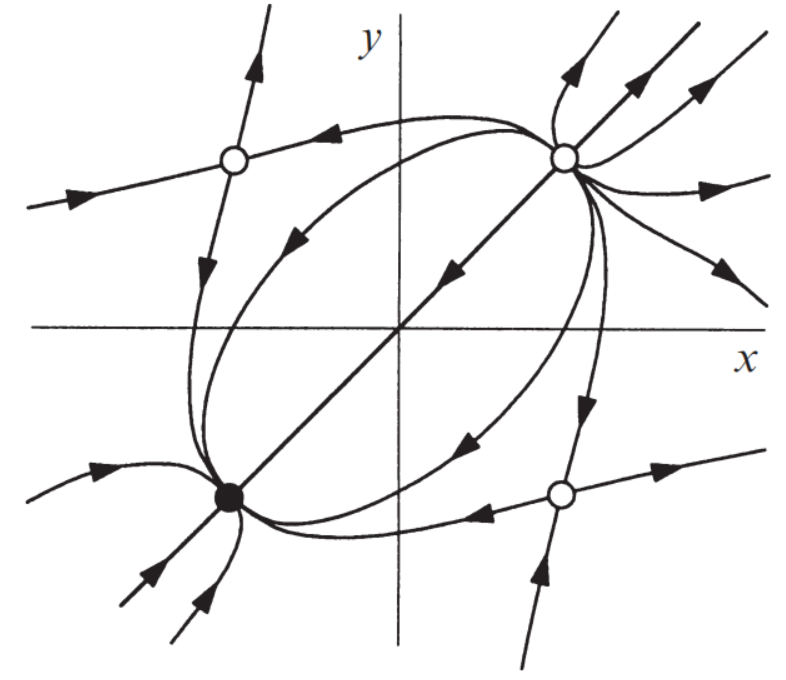
\includegraphics[width=0.4\linewidth]{fig667.jpg}
	\end{figure}
\end{frame}
% -----------------------------------------------------------------------------
\end{document}
